\chapter{Einleitung}
\label{cha:Einleitung}

\section{Zielsetzung}
Diese Bachelorarbeit dient als Vorarbeit für die Re-Implementierung einer existierenden Maillösung  der Frima curecomp GembH, wobei in dieser Arbeit der Fokus auf die Re-Implementierung des Designs gelegt wird. Diese Arbeit wird aufzeigen wie das existierende System in seinen Bereichen wie Client API, Datenbank Integration und das Erstellen der E-Mails, in weitere Folge 'E-Mail Vorlagen' genannt, funktioniert und designt wurde. Dieses existierende Design wird analysiert und ein Verbesserungsvorschlag eingebracht wie ein mögliches neues Designs aussehen könnte. Die Konzepte der Implementierung wie die verwendeten Pattern, die Grundlage der Designentscheidung sowie deren Vorteile und Nachteile werden diskutiert. \\\\
Da meiner Meinung nach die existierende Implementierung einige Mängel und Designfehlentscheidungen beinhaltet und dadurch weder flexibel noch erweiterbar ist, wurde der Fokus dieser Arbeit auf das Design dieser Maillösung und dessen Verbesserung gesetzt, wobei diese Arbeit wiederum als Grundlage für die praktische Bachelorarbeit dienen soll, die die Umsetzung der hier entwickelten und diskutierten Konzepte beinhalten soll. \\\\
Als Unterstützung wurden folgende beiden literarischen Werke gewählt:
\begin{enumerate}
	\item Refactoring to patterns\footnote{Author: Joshua Kerhievsky, ISBN: 0-321-21335-1}
	\item Refactoring Databases\footnote{Author: Scott W.Ambler/Pramod J.Sadalage, ISBN: 0-321-29353-3} 
\end{enumerate}
\section{Ist-System}
Im folgenden wird das existierende Design der Implementierung in den drei Bereichen
\begin{enumerate}
	\item \emph{Client-API}\\
	      Wie versenden bzw. generieren die Systeme die E-Mails
	\item \emph{Datenbank Integration}\\
	      Wie ist das Datenbankdesign und welche Daten werden gespeichert und warum
	\item \emph{E-Mail Vorlagen}\\
	      Wie werden die Inhalte der E-Mail generiert bzw. erstellt.
\end{enumerate}
Da der Mailversand in Java verhältnismäßig einfach ist wird auf diesen Teil nicht genauer eingegangen sehr wohl aber die Funktionalität im weiteren Verlauf dieser Arbeit diskutiert. \
Die oben genannten drei Unterteilungen stellen die Hauptteile der Maillösung dar und werden auch in einem neuen Design so benötigt ohne Rücksichtnahme auf die konkrete Art der Implementierung.
\begin{figure}[h]
\centering
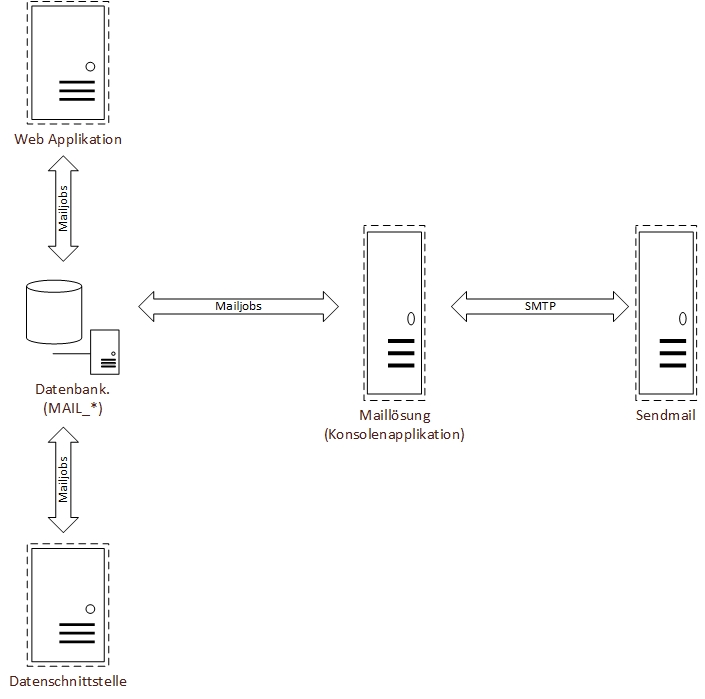
\includegraphics[scale=0.40]{Systemaufbau_alt.jpg} %{CS0031}
\caption{Diese Abbildung zeigt den konzeptionellen Aufbau der existierenden Maillösung und den jetzigen Kommunikationsweg zwischen den Systemteilnehmern}
\label{fig:systemaufbau-alt}
\end{figure}
\newpage
In dieser Abbildung können wir sehen dass es nur einen Kommunikationsweg zwischen den Systemteilnehmer gibt und zwar die Kommunikation über die Datenbank. Dies bedeutet es werden sogenannte Mailjobs erstellt, die einen Eintrag in einer Tabelle der Datenbank darstellen, welche alle Daten für die E-Mail zur Verfügung stellen und von der Maillösung ausgelesen und verarbeitet werden.\\
Hierbei enthält die Maillösung alle Vorlagen für alle implementierten E-Mails und SQL Abfragen, die die Daten aus der Datenbank auslesen und diese ausgelesenen Daten als Parameter and das Vorlagensystem weitergibt damit dieses die tatsächliche E-Mail Nachricht erstellen kann. Hierbei ist die Aktualität der Daten kritisch, da die E-Mail zeitversetzt zum erstellten Mailjob generiert wird und sich dadurch auch die Daten, die aus der Datenbank ausgelesen werden, sich zwischenzeitlich ändern könnten. Ebenso müssen die Daten separat und meistens erneut aus der Datenbank ausgelesen werden, obwohl in den meisten Fällen die Daten beim Erstellen des Mailjobs bereits vorhanden und vor allem zu diesem Zeitpunkt auch aktuell waren. Es gibt zwar Fälle in denen zeitgesteuert E-Mails generiert werden, wie z.B.: einmal täglich Lieferverzugsmeldungen, in denen der aktuelle Status der Datenbank eine Rolle spielt. Dieser Typ der E-Mails stellt jedoch im Verhältnis zu den \emph{'sofort versendeten'} E-Mails nur einen kleinen Prozentanteil dar und hier ist das Problem der Aktualität der verwendeten Daten nicht vorhanden. Bezüglich der Aktualität der Daten sei noch angemerkt dass das erneute Versenden einer E-Mail im bestehenden System nicht mit konsistent Daten möglich ist, da die Daten jedes mal erneut aus der Datenbank ausgelesen werden und der ursprüngliche Zustand der Daten nicht garantiert zur Verfügung steht, da diese sich zwischenzeitlich hätten ändern können, was auch nicht nachvollziehbar wäre.
\subsection{Client-API}
Da die Kommunikation ausschließlich über die Datenbank erfolgt ist eine echte Client API nicht vorhanden. Alle Systeme implementieren das Erstellen der Mailjob Einträge selbstständig und es wird keine gemeinsame Client API verwendet, was einen gewissen Grad der Inkonsistenz bei Änderungen der Datenstruktur sowie der Semantik der Daten mit sich bringt. Als Beispiel wird hier die Semantik der einzelnen Spalten angeführt, die zwar technisch sich innerhalb einer Datentyp Domain befinden, sich die semantische Bedeutung der enthaltenen Daten aber unterscheidet. Dies ist zwar Teil der Datenbank Integration aber die Tatsache dass diese Semantik rein innerhalb der Applikation abgebildet werden kann und nicht über die Datenbankfunktionalitäten wie z.B.: Fremdschlüssel wird dieser Teil hier diskutiert. Da die Maillösung über SQL Abfragen die Daten für die E-Mail Nachricht erhält müssen auch Parameter bereitgestellt werden, die in der SQL Abfrage gesetzt werden. Diese Parameter wurden \emph{'generisch'} über eine festgesetzte Anzahl von Tabellenspalten abgebildet, dessen enthaltene Daten je nach E-Mailtyp anders interpretiert werden. Es kann also sein das ein Eintrag einer Tabellen für die Spalte \emph{COL\_1} einen String enthält mit dem Wert \emph{'Thomas Herzog'} und ein anderer Eintrag einen string mit dem Wert \emph{'14'} der in der SQL Abfrage aber als Integer Datentyp behandelt wird. Die Systeme die Mailjobs erzeugen müssen sich also dem Kontext einer E-Mail bewusst sein, sowie müssen berücksichtigen, dass die richten Spalten der Tabelle \emph{MAIL\_JOB} mit den richtigen Daten befüllt werden, wobei auch beachtet werden muss in welchen Datentyp der Datensatz in weiterer Folge durch die Mailösung interpretiert wird.\\
Dies ist in meinen Augen sehr inkonsistent und fehleranfällig und hat auch schon einige Probleme verursacht.\\\\
\begin{figure}[h]
\centering
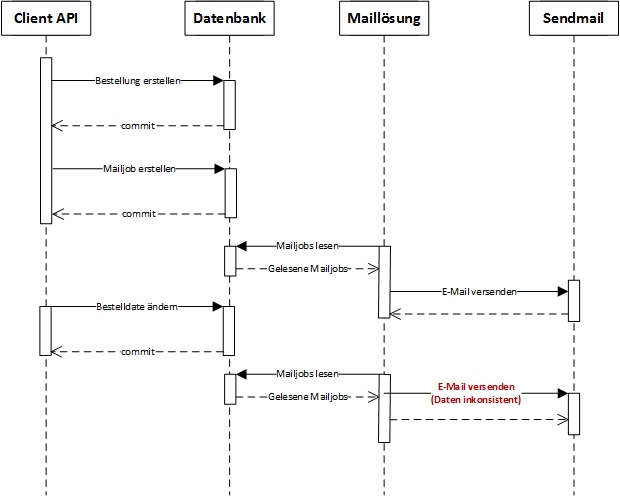
\includegraphics[scale=0.70]{Emailvesand_Client_Api.jpg}
\caption{Diese Abbildung zeigt das Problem der inkonsistenten Daten beim erneuten E-Mailversand einer bereits versendeten E-Mail, mit dem Beispiel einer angelegten und anschließend geänderten Bestellung, auf}
\label{fig:systemaufbau-alt}
\end{figure}
\newpage



\subsection{Datenbank Integration}
\subsection{E-Mail Vorlagen}
\section{Soll-System}
\subsection{Client-API}
\subsection{Datenbank Integration}
\subsection{E-Mail Vorlagen}